%
% Modified by Sameer Vijay
% Last Change: Wed Jul 27 2005 13:00 CEST
%
%%%%%%%%%%%%%%%%%%%%%%%%%%%%%%%%%%%%%%%%%%%%%%%%%%%%%%%%%%%%%%%%%%%%%%%%
%
% Sample Notre Dame Thesis/Dissertation
% Using Donald Peterson's ndthesis classfile
%
% Written by Jeff Squyres and Don Peterson
%
% Provided by the Information Technology Committee of
%   the Graduate Student Union
%   http://www.gsu.nd.edu/
%
% Nothing in this document is serious except the format.  :-)
%
% If you have any suggestions, comments, questions, please send e-mail
% to: ndthesis@gsu.nd.edu
%
%%%%%%%%%%%%%%%%%%%%%%%%%%%%%%%%%%%%%%%%%%%%%%%%%%%%%%%%%%%%%%%%%%%%%%%%

%
% Chapter 3
%

\chapter{TWO PROTON TRANSFER AT NOTRE DAME}
\label{chap:2pExpt}

\begin{comment}
Give an overview of the requirements for two-proton transfer and say that ND has a buncher and a Tandem accelerator that goes up to 10 MV so we can get beam energies up to 30 MeV for \He{3} and we have a beamline with a long flight path SO we can do this experiment.
\end{comment}

The previous chapter demonstrated the interest in studying \reaction ; this chapter will discuss the beam production and experimental setup.  The most important peices of the setup are the beam energy, the beam bunching, and the optimization of the neutron detector to provide excellent timing information.   

% detecting neutrons
% this means we need timing information
% so the beam must be bunched
% and the detector must be built to give good timing
% and placed to give good timing
Measuring the time of flight (TOF) of the neutron to sufficient accuracy requires both beam bunching and a long neutron flight path.  In a continuous beam, there is no way to know which \He{3} was associated with a neutron event in the detector, and therefore no way to determine TOF.  Bunching the beam so that clumps of \He{3} arrive at the same time and providing a signal correlated to their arrival at the target allows a TOF measurement with a precision determined by the time-width of the bunch.  This limit on time resolution constrains the distance between the target and detector.  

% interested in 0+ distribution
% and there's an ideal beam energy for that
% and that constrains the distance between the target and neutron detector
As discussed in the previous chapter, the purpose of this experiment is to understand the distribution of the \zp state.  The maximum \zp cross-section for \reaction requires a beam energy near 18 MeV, but the resolution of the neutron detector decreases with increasing neutron energy.  The beam energy must be as close to 18 MeV as possible while still providing sufficient resolution.

States populated through different $l$ transfer can be discriminated by their angular distributions.  The DWBA calculations in the previous chapter show the expected maximum and minimum of the \zp cross-section to be at 0 and 22 degrees, respectively. 


\section{Beam Production at Notre Dame}
The beam delivered to the target is 16 MeV bunched \He{3}.  In this section, we will follow the beam through its production and acceleration.

The Helium Ion Source (HIS) provides negative \He{3} ions to the accelerator.  A duoplasmatron ion source filled with \He{3} gas uses a discharge across high voltage to convert some of the gas into plasma.  Electrostatic elements extract positive \He{3} ions from the plasma and accelerate them into a canal filled with lithium vapor.  Lithium is crucial to creating negatively charged beam because it donates electrons generously, and a small fraction of the \He{3} becomes negatively ionized after passing through the canal.  A dipole magnet after the ion source removes the carbon, oxygen, and other impurities that contaminate the \He{3} beam.  Movable, thick tungsten slits block much of the beam, allowing only beam within a small range of magnetic rigidity to pass through to the accelerator.

The accelerator at Notre Dame is a tandem Van deGraaff accelerator made by High Voltage Engineering Corporation.  Its maximum terminal potential is 10 MV.  Negatively charged beam enters and accelerates toward the positive terminal, located in the center of the machine. A thin carbon foil ($\sim$ 3 $\mu$g/cm$^2$) in the center of the machine strips electrons from the beam.  The now-positive beam accelerates again, away from the positive terminal. In general, the final energy of a particular beam with is 

\begin{equation}
E = E_{HIS} + (1+q)eV_T
\end{equation}

where $V_T$ is the terminal voltage, $E_{HIS}$ is the energy of the beam exiting the HIS, and $q$ is the charge state of the beam after passing through the carbon foil.  \He{3} beam is fully stripped of its electrons by the carbon foil, and so the terminal voltage required to produce 16 MeV \He{3} is 5.33 MV, a comfortable operating voltage for the accelerator.  The beam leaving the accelerator has an energy spread on the order of the terminal ripple and is tightly focused, but it must arrive focused on the target, which is ?? m away.  To produce a focused, near-monoenergetic beam at the target, beam selection using dipoles and slits and also focusing elements are necessary.  These will be discussed in the next section.


\subsection{Beam Focusing and Selection}

Dipole magnets can select beam based on rigidity; since the mass and charge of the desired beam are fixed, a dipole acts as a momentum filter.  A large dipole magnet with beam-stopping slits at its exit leaves the beam with an energy spread of only 10 keV.  The magnetic field strength is calibrated against the nuclear magenetic resonance (NMR) of hydrogen. 

The accelerated beam must travel in vacuum from the accelerator to a target.  Many focusing and steering elements along the way are necessary to obtain a reasonable transmission rate.  Two Einzel lenses [need cite] focus the beam before it enters the accelerator, and a set of electrostatic steerers before and after the accelerator are enough to position the beam before it enters the energy-selecting dipole magnet.

Quadrupole doublet magnets focus the beam as it travels through the target rooms, and another set of steerers allows correction of the beam position and angle.  The final focusing element before the target are two large-bore, variable-strength solenoid magnets [cite needed] that focus the beam to a spot approximately 2 mm in diameter.

% figure: beamline
\begin{figure}[htp]
\centering
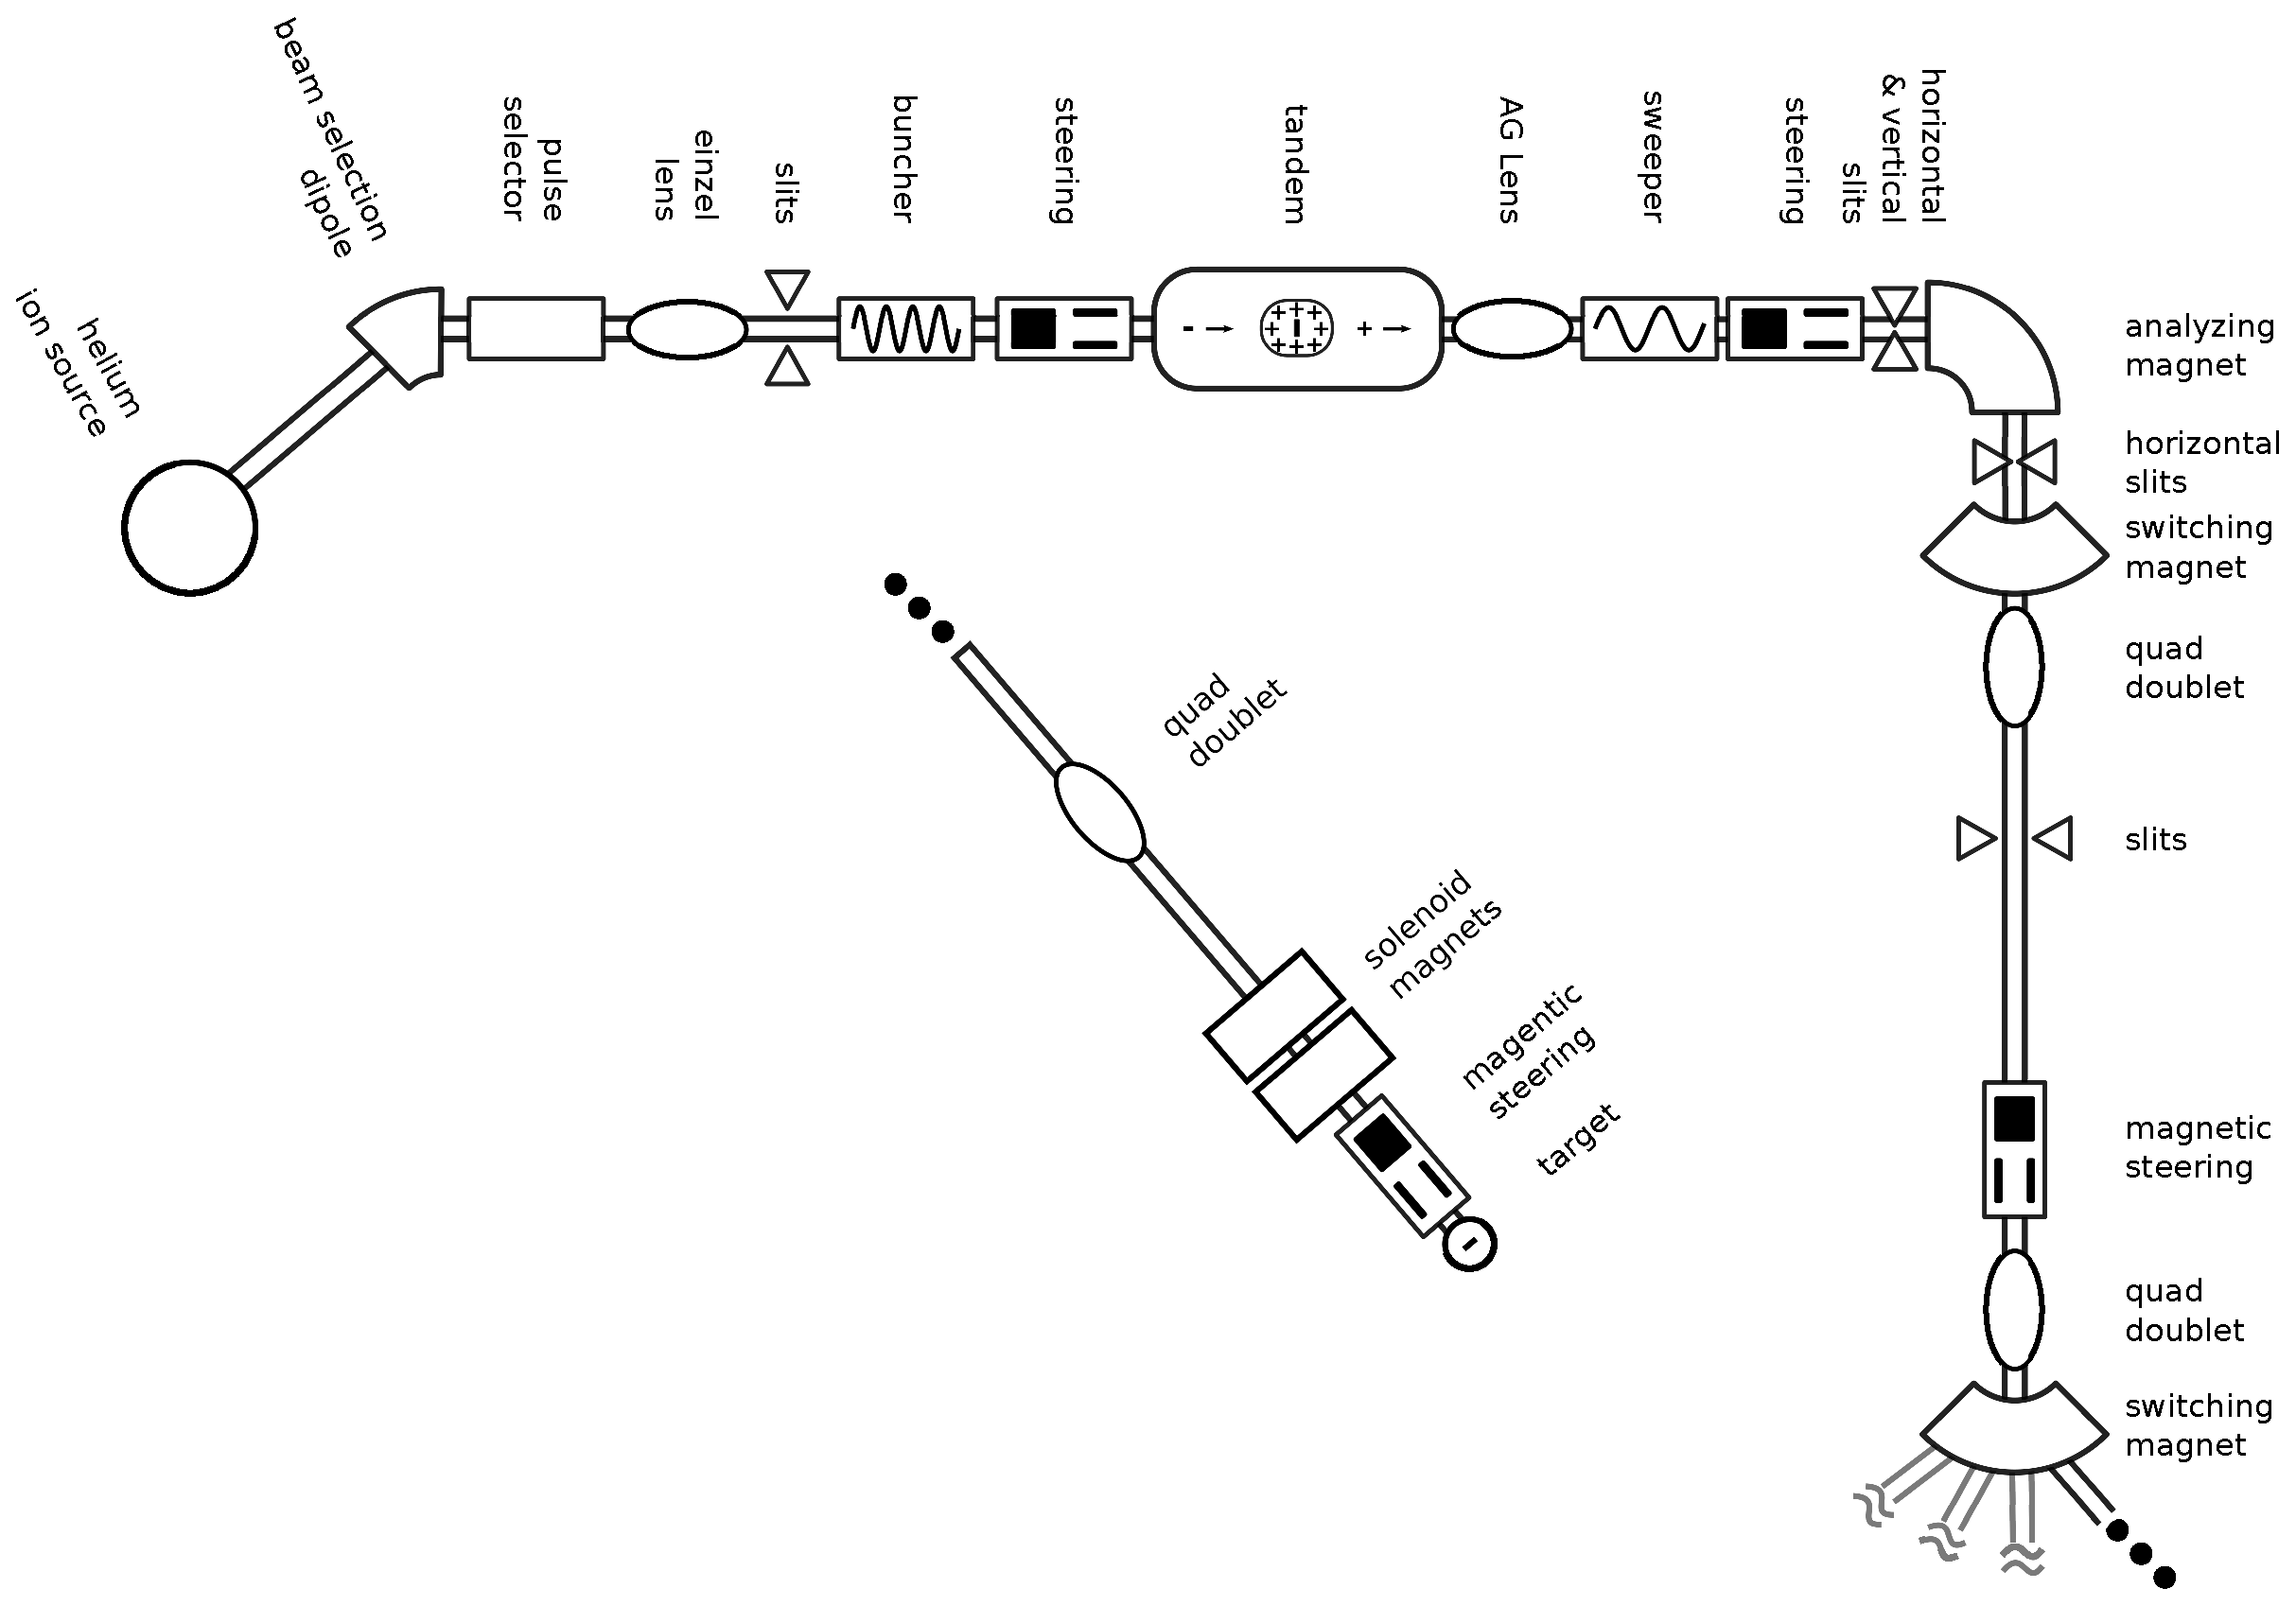
\includegraphics[width=1.0\textwidth]{figures/NSL_beamline.eps}
\label{fig:beamline}
\caption{Beam production at Notre Dame.}
\end{figure}

\subsection{Beam Bunching}

Continuous beam would make it impossibile for our detectors to determine the neutron TOF.  It is possible to bunch the beam so that ``bunches'' of \He{3} arrive at the target, each bunch having a time spread of approximately one ns. There are three components to the bunching system at Notre Dame.  The first is the buncher itself, which slows down particles that would arrive too early at the target and speeds up particles that would arrive too late.  The buncher is not able to group all of the incoming beam into bunches; about 40\% of the beam is pushed into a discrete bunch, while the remaining 60\% is a continuous background.  Any beam background not associated with a bunch would, again, make determing neutron TOF impossible.  The sweeper removes this continuous background.  Together, the buncher and sweeper provide one ns bunches of beam separated by 100 ns, with no beam in between.  Because some of the slow neutrons coming from the reaction have TOF in excess of 300 ns, a pulse-selector is used to eliminate three out of every four bunches.  The buncher, sweeper, and pulse-selector together provide clean bunches of beam separated by 400 ns.  The rest of this section describes how each of these components works.

The beam buncher at Notre Dame works by slowing down particles that would arrive too early at the target and speeding up particles that would be arriving too late.  To acheive this, two grids perpendicular to the beam connect to a radiofrequency (RF) power supply to create an intense electric field that varies in time.  If the electric field were a sawtooth wave in time, the beam bunches would contain all the beam \cite{LynchBunching}.  Commercially available RF power supplies providing adequate current and rapid enough signal, however, generally vary sinusoidally in time.  At Notre Dame, a single frequency buncher that operates at 9.85 MHz is used.  The best bunching occurs while the RF signal is increasing approximately linearly with time; when the electric field is decreasing, de-bunching occurs.  At the target, nanosecond (ns) wide bunches contain $\sim$40\% of the beam and arrive at the target every 101 ns on top of the remaining continuous beam.  This continuous beam would render our time signal useless and must somehow be removed.

% figure: how a beam buncher works
\begin{figure}[htp]
\centering
\includegraphics[width=1.0\textwidth]{figures/beamBunching.eps}
\label{fig:bunching}
\caption{Beam bunching using a varying electric field.}
\end{figure}

The ``sweeper'' provides a sinusoidal electric field that is timed to deflect the continuous beam between the bunches.  A set of vertical slits immediately after the sweeper stops the deflected beam.  The timing between the buncher and the sweeper must be adjusted carefully.  Even a few-nanosecond change in the timing can affect which portion of the beam is swept away. 

%figure of beam profile and sweeper

It is possible to take data without pulse selection, but because the spread in TOF of the neutron spectrum is in excess of 200 ns, it complicates the TOF spectrum considerably.  With bunches arriving at the target every 100 ns, it will be impossible to tell if a neutron is very fast and associated with the current bunch or very slow and associated with the previous bunch.  The resulting spectrum is shown in Figure \ref{fig:PSvsNPS_TOF}.

% figure: the considerably complicated spectrum
\begin{figure}[htp]
\centering
\subfloat[][]{
   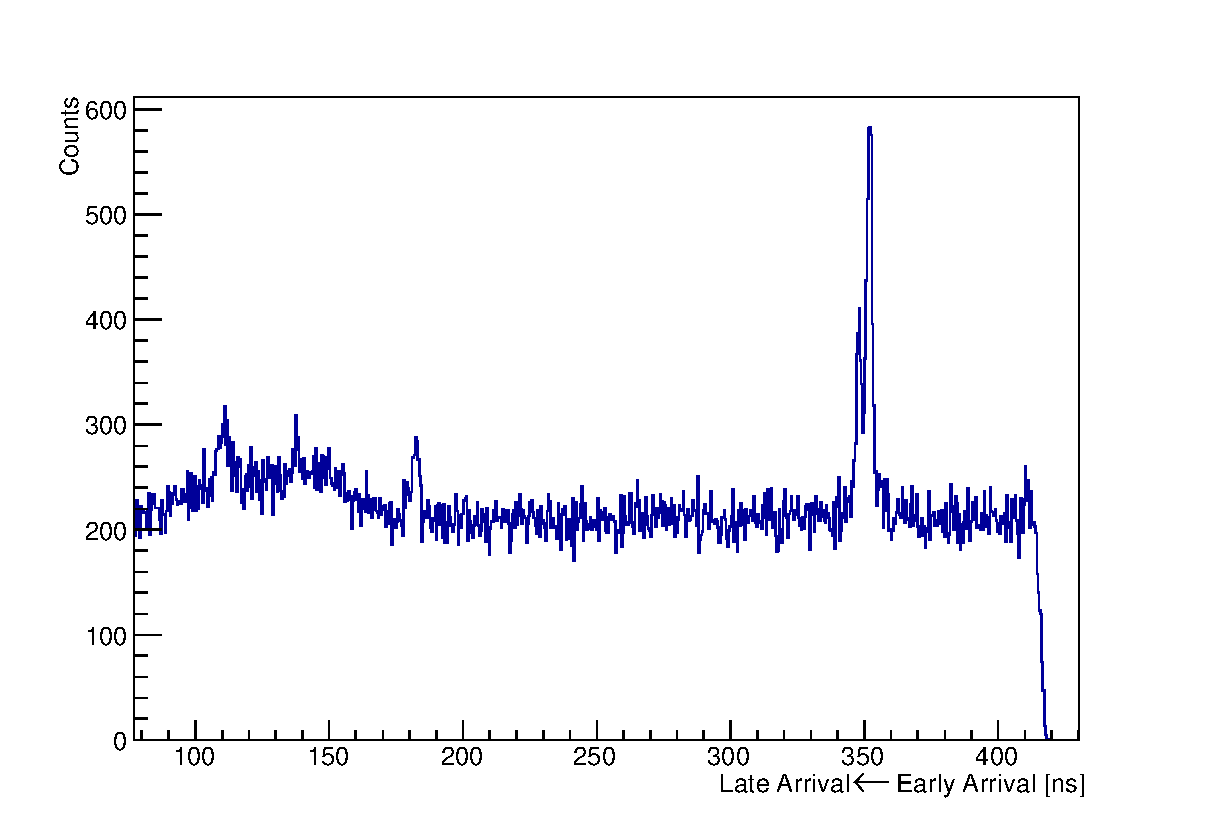
\includegraphics[width=0.4\textwidth]{figures/PS_BarA_Sep.eps}	
}
\subfloat[][]{
	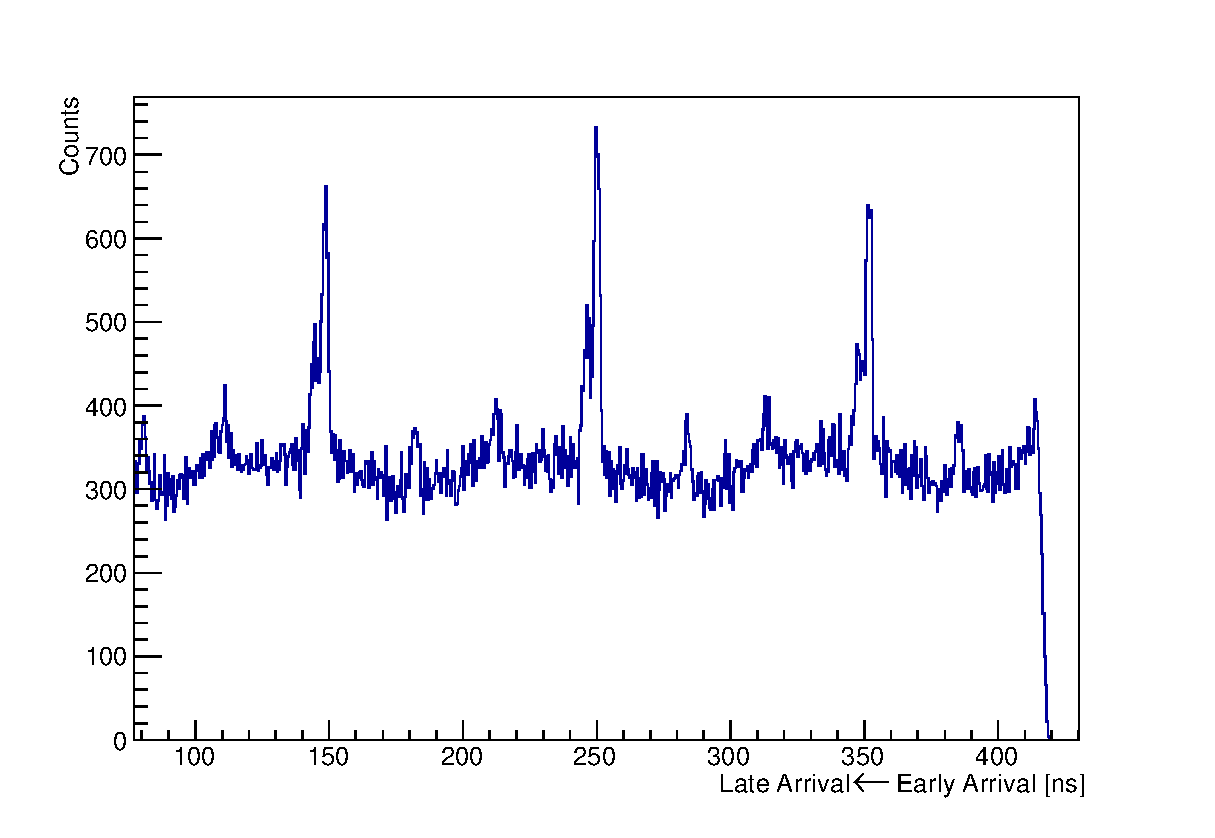
\includegraphics[width=0.4\textwidth]{figures/NPS_BarA.eps}
}
\label{fig:PSvsNPS_TOF}
\caption{Figure A shows timing spectrum from a pulse-selected beam.  The timing spectrum in figure B is from beam with no pulse selection.  Both timing spectra are from a \He{3} beam on a \Ge{76} target.}
\end{figure}

To give all the neutrons resulting from one beam bunch time to reach the detector before the next bunch strikes, a ``pulse selector'' eliminates three of every four bunches, resulting in 400 ns between each bunch at the cost of beam intensity.  The pulse selector is located before the accelerator and consists of two parallel plates, one held at ground and the other at +400 V.  A fast switch (SCR) connects the high-voltage plate to ground, letting the selected bunch through without deflection.  While the beam width is only one ns at the target, at the sweeper the bunch is approximately 80 ns wide, so the SCR must hold the plate at ground for 80 ns to let the entire bunch through.

% figure: slow neutrons and their dissappearance

Beam bunching and pulse selection reduces available beam - the swept beam current is only 40\% $\times$ $\frac{1}{4} = 10$\% of the non-bunched current.  But without bunched beam it would not be possible to distinguish the neutrons of interest in the (\He{3},n) transfer reaction.  As it happens, however, the Notre Dame facility cannot improve the statistics of this experiment by very much because the radiation limits on the room with the detector are so low that even with pulse selection, the beam is near its maximum allowed current.

\section{The Target Chamber}
\begin{comment}
target
thin stainless stell wall
Si detector
BaF2 detector
\end{comment}

The 16 MeV \He{3} beam has been bunched, swept, pulse-selected, and steered and focused onto the target.  The bunches that were 80 ns wide have converged into 1 ns wide bunches.  To maintain the energy resolution of the beam, the gold-backed Ge targets are positioned so that the first material the beam encounters is Ge.  Resulting neutrons can pass through the gold without the energy straggling that would afflict the \He{3} were it to pass through the gold.  

To measure the absolute scale of the cross-section, it is necessary to know the number of particles incident on the target.  This is done in several ways.  The most precise measure of the number of incident particles is a Si detector placed in the target chamber, positioned to measure \He{3} scattered off the gold backing of the Ge targets.  Because the \Mg{26} target is self-supporting, it is necessary to record other measures of the beam.  One indicator of the beam current is the charge measured from an electrically isolated beamstop downstream of the target.  Another measure of the beam current is a NaI2 detector located just outside the chamber, which is sensitive to $\gamma$ radiation produced by beam interactions in the target.  

In addition to knowing the number of incident particles, it is also necessary to know the particle density of the target.  The target thickness is well-known from RBS measurements; the results are summarized in Chapter ?? and a description of the analysis is in Appendix ??.  


\section{The Neutron Detector}
\begin{comment}
Discuss neutron wall briefly.  Can reference NIMA paper. Explain why it's important that it's wide-angle. 
\end{comment}

The resulting products of a two-proton transfer onto \Ge{76} are a neutron and a \Se{78} nucleus.  Charged particle detection is highly efficient, but the heavy, charged \Se{78} nucleus is unlikely to escape the target, forcing us to rely on neutron detection to study this reaction. To study the neutrons, the detector must provide many hydrogens - protons for the neutrons to interact with.  The detector must also be far away from the target, to allow a TOF that gives sufficient neutron energy resolution.  And the detector must be positioned to be sensitive to the \zp states of interest.  Because the \zp states peak at 0 degrees and drop to a minimum at 20 degrees, the detector must span these angles.

The neutron detector consists of 16 large (1.5 m $\times$ 0.15 m $\times$ 0.05 m) bars of commercially available scintillator [reference BC408?].  The detectors sit in a circle of radius 14.6 m centered around the target.  The forwardmost angle relative to the beam is 5$^{\circ}$ and the largest angle is $21^{\circ}$.  Ideally, the detectors would extend to 0$^{\circ}$, but a concrete support beam makes this impossible.  At this distance, the solid angle subtended by each detector is only 10 cm/15 m $\times$ 2.5 m/15 m = 0.11 sr.

% figure - picture of detector

Each plastic scintillator bar is equipped with two photomultiplier tubes (PMT's) with signal risetimes of approximately 5 ns.  Because the PMT's have such a fast risetime, they provide excellent timing information as well as energy information.  Energy deposited is not useful for neutron identification; it is timing information that indentifies neutrons.  If the neutron always deposited its full energy in the detector, the energy spectrum would show sharp peaks corresponding to each neutron energy.  However, a neutron interacting with a proton only transfers all its energy to that proton in a head-on collision, which rarely occurs.  Much more likely is a glancing interaction, where the neutron imparts only some of its energy to the proton.  The energy spectrum of monoenergetic neutrons ranges from the detector threshold up to the neutron's full energy, making it impossible to determine the energy of the neutron from its deposited energy.  Instead, the TOF is used to separate neutron of differing energies.  This is why the detectors fast-risetime PMT's instrument the detectors; it is the timing information that determines the energy resolution.  The PMT signal processing is discussed further in the electronics section.

% figure of charged-particle energy spectrum
% figure of neutron energy spectrum

We have said that timing information is the useful information given by our neutron detectors, and that the flight path between the target and detectors must be long to ensure reasonable resolution.  What resolution is reasonable for this experiment?  And how long a flight path is needed for such a resolution?  A 16 MeV \He{3} can populate many excited states in \GeTargets; an excellent resolution would allow separation between the ground and first excited state.  Since the beam bunch itself has a width of 1 ns, the flight path would need to be long enough that the TOF of the ground and excited state neutrons differs by at least 1 ns. Conservation of energy and momentum determines the time $t$ it takes for a neutron with relativistic momentum $p$ to travel the distance $d$ between the target and the detector.

% figure: \Ge{76}, 74Ge level scheme

\begin{equation}
t(p) = \frac{d}{v} = d\times\sqrt{\frac{m^2+p^2/c^2}{p^2}}
\end{equation}

\begin{equation}
t(p_1) - t(p_2) = 1 ns = d\times(\sqrt{\frac{m^2+p_1^2/c^2}{p_1^2}}-\sqrt{\frac{m^2+p_2^2/c^2}{p_2^2}})
\label{eq:TOF}
\end{equation}

In the case of \Ge{76},  the energies of the ground and first excited state neutrons differ by only 0.5 MeV out of $\sim$22 MeV.  At this energy, a flight path of 14.6 m gives a time difference between these two neutrons of ?? ns, very close to the intrinsic width of the bunch.  While a longer flight path would improve resolution, this resolution is typical of TOF experiments [CITE] and certainly allows separation of the ground state from the higher excited states.  

\subsection{Electronics}
\begin{comment}
Electronics diagram!  Discuss two most important aspects: TDC and ADC from phototubes
\end{comment}

In principle, the timing information is all the data acquisition (DAQ) needs to record.  This would be true if there were no background radiation, but concrete in the room emits low-energy $\gamma$ radiation that leaves signal in the detector at a high rate.  Measuring the energy deposition is necessary because it allows us to eliminate this low-energy background radiation.

While energy information is necessary, it does not need to be terribly precise.  The timing information, however, is the only information useful for neutron identification and must be as precise as possible.  The goal for the electronics is to not add spread to the timing that is noticable above the timing spread already inherent in the beam bunching.  This is why the detectors are equipped with PMT's that have excellent timing response.  The 5 ns PMT signal risetime, together with Constant Fraction Discriminators (CFD's), give timing information with jitter that is about 1 ns.

% figure: CFD operation

When a real event occurs in some bar of the neutron detector, the DAQ must record the energy and time of both the top and bottom PMT of that bar.  A charge to digital converter (QDC) can integrate the PMT signal and a time to digital converter (TDC) can measure the time between a logic pulse created by the PMT signal and the logic pulse from the beam buncher.  Because time resolution is crucial, constant fraction discriminators (CFD's) and not leading edge discriminators create the logic pulse sent to the TDC.  

The lone signal provided by the PMT base is not adequate for this processing because the QDC and TDC are destructive measurements and therefore require separate signals.  The signal from the PMT base is also too small to trigger the CFD's.  A $\times$10 amplifier makes the signal large enough to trigger the CFD's and provides two copies of the input signal, one which can be analyzed for timing information while the other is analyzed for energy information.  A simplified diagram of the data acquisition is shown in fig \ref{fig:simpleElectronics}.

% figure: simple electronics
\begin{figure}[htp]
\centering
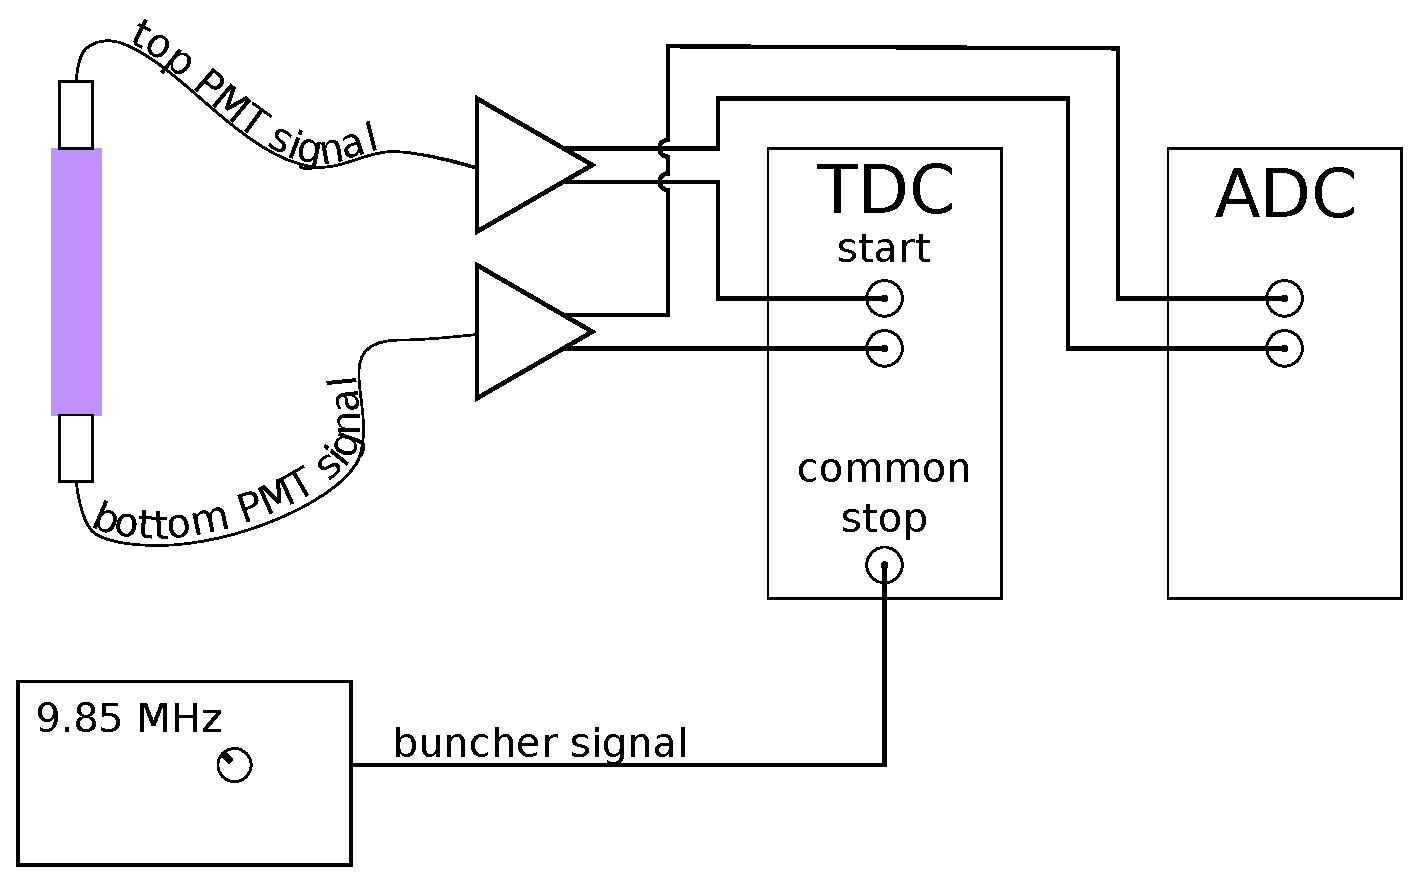
\includegraphics[width=1.0\textwidth]{figures/basic_electronics.eps}
\label{fig:simpleElectronics}
\caption{A simplified diagram of the neutron detector electronics showing the acquisition of timing and energy information from the detectors.}
\end{figure}

The fundamental components of the DAQ are the TDC, the QDC, and the event trigger that causes the DAQ to read each module.  For just one neutron detector, triggering any time the top or bottom PMT fired would waste the DAQ with recording many noise events.  A real event should create signals in both the top and bottom PMT's, and requiring a coincidence between the two results in a reasonable trigger.  One way to define an event trigger for the entire neutron wall, then, would be to trigger any time a coincidence between associated top and bottom PMT's occurs.  But constructing this trigger with NIM logic units requires many separate logic gates and is unnecessarily complicated.  

One solution is to use the built-in OR of the CFD.  Instead of requiring a top and bottom signal in the same bar, the condition is loosened to requiring a signal in a top PMT and a bottom PMT in the same eight-bar group.  Each CFD is an eight-fold unit that receives only top or bottom signals and provides an OR output.  The presence of some top signal AND some bottom signal triggers the event signal.  Such an event only requires that both a top and a bottom signal coincided but does not require that these signals belonged to the same bar.  Such an event trigger includes all events of interest, where the top and bottom signal belong to one bar, but also includes spurious events where no bar has signal in both its top and bottom PMT.  With a dead time of less than 30\%, this event condition does not hinder data collection, and simple software cuts eliminate spurious events.

% figure: event trigger
\begin{figure}[htp]
\centering
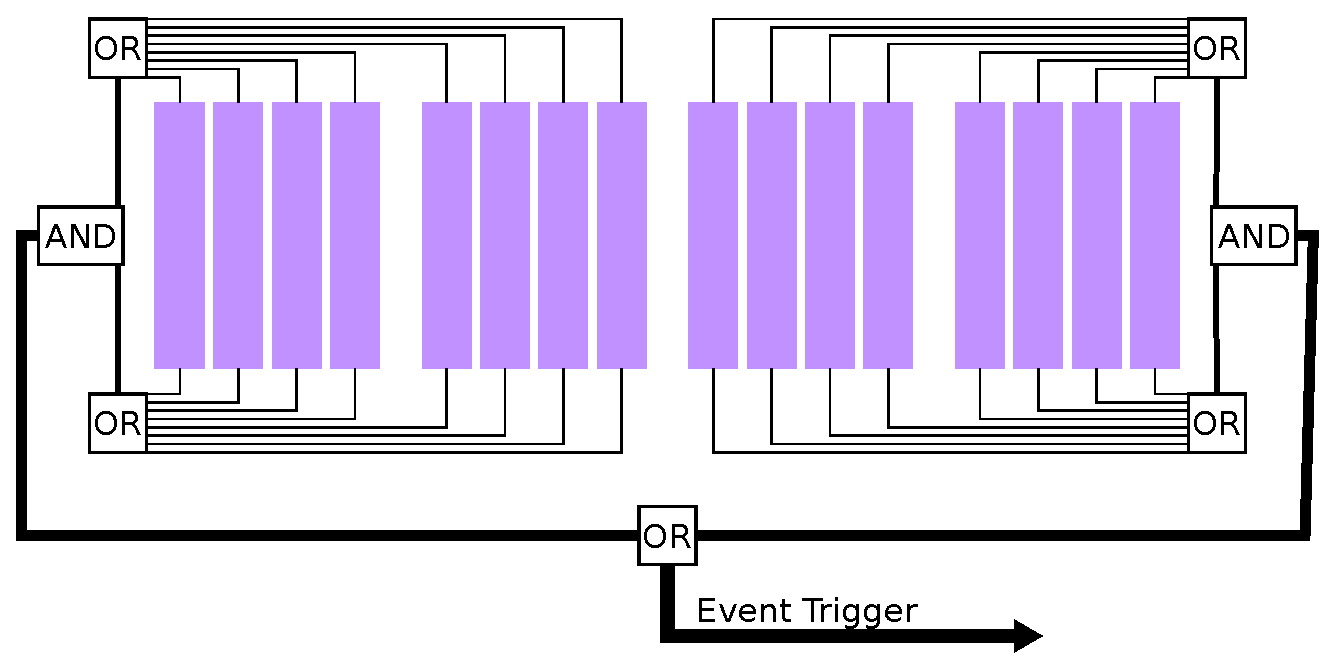
\includegraphics[width=1.0\textwidth]{figures/event_trigger.eps}
\label{fig:eventTrig}
\caption{The event trigger for the DAQ requires a coincidence between a top PMT and a bottom PMT from the same group of eight detectors.}
\end{figure}

% discuss energy, time info from near-target detectors
% and then scalers?
The time information, energy information, and a signal to indicate that this information should be read from the modules and recorded, form the core of the DAQ.  There are other quantities, however, the DAQ must record.  One of these is the dead time; the DAQ cannot collect new events while it is processing an event, and the live time is the appropriate time to use in cross-section calculation.  The DAQ itself provides two signals that allow us to measure the live time: a 100 Hz signal and a NIM logic pulse that is low when the DAQ is busy.  Vetoing the timing signal with this busy signal and recording both the un-vetoed 100 Hz signal and the busy-vetoed signal gives the ratio of live time to dead time.  The schematic is shown in figure ??.

The DAQ must also record information from the detectors near the target.  The particles of interest for the Si detector are deflected \He{3} beam, and because they are charged and deposit all their energy in the Si detector, the energy is a useful way to identify \He{3} and should be recorded.  The NaI2 detector sits outside the target chamber and will only see escaping neutron and $\gamma$ radiation; timing, not energy, information is the useful quantity.  Finally, because these detectors sit so close to the target, their event rate is much higher than that of the neutron detectors.  While these 'witness' detectors are essential to determining the absolute particle flux through the target, the dead time they cause the DAQ should not prohibit events from the neutron detector itself from being recorded.  Running the signals from the Si and NaI2 through a pre-scaler before adding it to the event trigger limits the dead time contribution of these detectors to less than 20\%.

% figure: Si, Q.live, NaI accumulation

% figure: full electronics

% % uncomment the following lines,
% if using chapter-wise bibliography
%
% \bibliographystyle{ndnatbib}
% \bibliography{example}
